\begin{center}
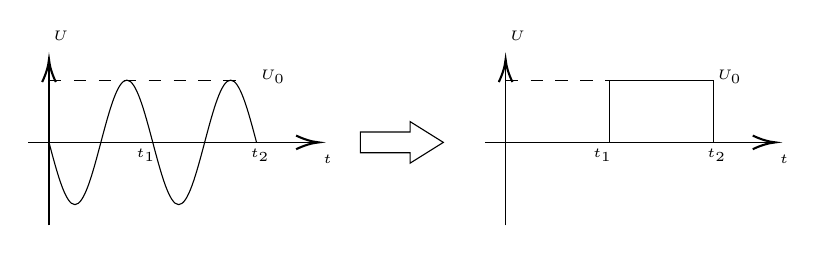
\begin{tikzpicture}[x=0.75pt,y=0.75pt,yscale=-1,xscale=1]
%uncomment if require: \path (0,300); %set diagram left start at 0, and has height of 300

%Shape: Wave [id:dp5957275904614414] 
\draw   (40,100) .. controls (44.08,115.37) and (47.98,130) .. (52.5,130) .. controls (57.02,130) and (60.92,115.37) .. (65,100) .. controls (69.08,84.63) and (72.98,70) .. (77.5,70) .. controls (82.02,70) and (85.92,84.63) .. (90,100) .. controls (94.08,115.37) and (97.98,130) .. (102.5,130) .. controls (107.02,130) and (110.92,115.37) .. (115,100) .. controls (119.08,84.63) and (122.98,70) .. (127.5,70) .. controls (132.02,70) and (135.92,84.63) .. (140,100) ;
%Straight Lines [id:da8807380521016539] 
\draw    (30,100) -- (168,100) ;
\draw [shift={(170,100)}, rotate = 180] [color={rgb, 255:red, 0; green, 0; blue, 0 }  ][line width=0.75]    (10.93,-3.29) .. controls (6.95,-1.4) and (3.31,-0.3) .. (0,0) .. controls (3.31,0.3) and (6.95,1.4) .. (10.93,3.29)   ;
%Straight Lines [id:da7234210438419781] 
\draw    (40,140) -- (40,62) ;
\draw [shift={(40,60)}, rotate = 90] [color={rgb, 255:red, 0; green, 0; blue, 0 }  ][line width=0.75]    (10.93,-3.29) .. controls (6.95,-1.4) and (3.31,-0.3) .. (0,0) .. controls (3.31,0.3) and (6.95,1.4) .. (10.93,3.29)   ;
%Straight Lines [id:da8881692477795176] 
\draw  [dash pattern={on 4.5pt off 4.5pt}]  (40,70) -- (130,70) ;
%Straight Lines [id:da7037740098329359] 
\draw    (250,100) -- (388,100) ;
\draw [shift={(390,100)}, rotate = 180] [color={rgb, 255:red, 0; green, 0; blue, 0 }  ][line width=0.75]    (10.93,-3.29) .. controls (6.95,-1.4) and (3.31,-0.3) .. (0,0) .. controls (3.31,0.3) and (6.95,1.4) .. (10.93,3.29)   ;
%Straight Lines [id:da24696901338014343] 
\draw    (260,140) -- (260,62) ;
\draw [shift={(260,60)}, rotate = 90] [color={rgb, 255:red, 0; green, 0; blue, 0 }  ][line width=0.75]    (10.93,-3.29) .. controls (6.95,-1.4) and (3.31,-0.3) .. (0,0) .. controls (3.31,0.3) and (6.95,1.4) .. (10.93,3.29)   ;
%Straight Lines [id:da028807109360900807] 
\draw  [dash pattern={on 4.5pt off 4.5pt}]  (260,70) -- (350,70) ;
%Right Arrow [id:dp35127513802390187] 
\draw   (190,95) -- (214,95) -- (214,90) -- (230,100) -- (214,110) -- (214,105) -- (190,105) -- cycle ;
%Straight Lines [id:da6668988615484821] 
\draw    (310,70) -- (310,100) ;
%Straight Lines [id:da5154013723623756] 
\draw    (360,70) -- (360,100) ;
%Straight Lines [id:da6769085058841795] 
\draw    (310,70) -- (360,70) ;

% Text Node
\draw (171,105) node [anchor=north west][inner sep=0.75pt]  [font=\tiny] [align=left] {$\displaystyle t$};
% Text Node
\draw (41,45) node [anchor=north west][inner sep=0.75pt]  [font=\tiny] [align=left] {$\displaystyle U$};
% Text Node
\draw (141,64) node [anchor=north west][inner sep=0.75pt]  [font=\tiny] [align=left] {$\displaystyle U_{0}$};
% Text Node
\draw (391,105) node [anchor=north west][inner sep=0.75pt]  [font=\tiny] [align=left] {$\displaystyle t$};
% Text Node
\draw (261,45) node [anchor=north west][inner sep=0.75pt]  [font=\tiny] [align=left] {$\displaystyle U$};
% Text Node
\draw (361,64) node [anchor=north west][inner sep=0.75pt]  [font=\tiny] [align=left] {$\displaystyle U_{0}$};
% Text Node
\draw (81,102) node [anchor=north west][inner sep=0.75pt]  [font=\tiny] [align=left] {$\displaystyle t_{1}$};
% Text Node
\draw (136,102) node [anchor=north west][inner sep=0.75pt]  [font=\tiny] [align=left] {$\displaystyle t_{2}$};
% Text Node
\draw (301,102) node [anchor=north west][inner sep=0.75pt]  [font=\tiny] [align=left] {$\displaystyle t_{1}$};
% Text Node
\draw (356,102) node [anchor=north west][inner sep=0.75pt]  [font=\tiny] [align=left] {$\displaystyle t_{2}$};


\end{tikzpicture}

\end{center}